\documentclass{standalone}
\usepackage{quiver}
\usepackage[most]{tcolorbox}
\usepackage{xcolor}
\usepackage{minted}

\usemintedstyle{default}
\setminted{
  bgcolor=backcolor,
  linenos=true,
  fontsize=\footnotesize,
  highlightcolor=codehighlightcolor,
  %xleftmargin=20pt
}

%
% Customize colors
%
\definecolor{chapter-color}{cmyk}{1, 0.50, 0, 0.25}
\definecolor{link-color}{cmyk}{1, 0.50, 0, 0.25}
\definecolor{cite-color}{cmyk}{0, 0.7, 0.9, 0.2}
\definecolor{codegreen}{rgb}{0,0.6,0}
\definecolor{codegray}{rgb}{0.5,0.5,0.5}
\definecolor{codepurple}{rgb}{0.58,0,0.82}
\definecolor{backcolour}{rgb}{0.95,0.95,0.92}
\definecolor{codebgcolor}{RGB}{129, 139, 152}
\definecolor{codehighlightcolor}{RGB}{255, 230, 153}
%\definecolor{codegreen}{RGB}{0, 153, 0}
%\definecolor{codegray}{RGB}{127, 127, 127}
\definecolor{codeblue}{RGB}{102, 214, 237}
\definecolor{codekeyword}{RGB}{249, 36, 114}
\definecolor{codecomment}{RGB}{127, 127, 127}
\definecolor{backcolor}{RGB}{242, 242, 235}
\definecolor{linkcolor}{RGB}{102, 0, 0}
\definecolor{corange}{RGB}{255, 70, 0}
\definecolor{cyellow}{RGB}{209, 153, 0}
\definecolor{cblue}{RGB}{64, 128, 255}
\definecolor{cbrown}{RGB}{153, 102, 51}
\definecolor{cpink}{RGB}{255, 0, 255}
\definecolor{cred}{RGB}{255, 64, 0}
\definecolor{cgreen}{RGB}{0, 191, 0}
\definecolor{clightblue}{RGB}{191, 217, 255}
\definecolor{cturquois}{RGB}{0, 255, 255}
\definecolor{cpurple}{RGB}{128, 0, 255}
\definecolor{clightgreen}{RGB}{175, 255, 175}
\definecolor{clightgray}{RGB}{211, 211, 211}
\definecolor{clightpink}{RGB}{255, 175, 255}
\definecolor{cdarkblue}{RGB}{0, 0, 255}
\definecolor{cdarkred}{RGB}{255, 0, 0}
\definecolor{cdarkgreen}{RGB}{0, 255, 0}
\definecolor{cgray}{RGB}{153, 153, 153}

\definecolor{myblue}{RGB}{55, 126, 184}
\definecolor{myorange}{RGB}{255, 127, 0}
\definecolor{myred}{RGB}{228, 26, 28}
\definecolor{mypurple}{RGB}{152, 78, 163}
\definecolor{mygreen}{RGB}{77, 175, 74}
\definecolor{myyellow}{RGB}{255, 255, 51}
\definecolor{mybrown}{RGB}{166, 86, 40}
\definecolor{mypink}{RGB}{166, 86, 40}
\definecolor{mygray}{RGB}{153, 153, 153}


% inline code

% Inline code
% see https://tex.stackexchange.com/a/568900
\usepackage[most]{tcolorbox}

\tcbset{
  codebase/.style={
    enhanced,
    fontupper=\vphantom{Ägpyj}\fontfamily{qcr}\selectfont,
    colframe=white,
    frame style={opacity=0},
    colback=codebgcolor!12,
    nobeforeafter,
    tcbox raise base,
    shrink tight,
    extrude by=2pt,
  }
}

\newtcbox{\codebox}{codebase,      equal height group=A}
\newtcbox{\eqcodebox}{codebase,    equal height group=B}
\newtcbox{\fncodebox}{codebase,    equal height group=C}
\newtcbox{\codebreakbox}{codebase, equal height group=D}

%\def\code#1{\codebox{\texttt{#1}}}
%\def\code#1{\codebox{\mintinline[fontsize=\small]{text}{#1}}} % creates a intermediate file for EVERY \code command

\def\code#1{\codebox{#1}} % original
\def\eqcode#1{\eqcodebox{#1}} % original
\def\fncode#1{\fncodebox{#1}} % footnote code original

% for inline \code{blabla} pieces that extend over the line break. This to manually break the line. Replace \code{bla} with \codebreak{bla} in those cases
\def\codebreak#1{\linebreak \codebreakbox{#1}}

% \usepackage{soul}
% \def\code#1{\hl{\texttt{#1}}}
% \def\codebreak#1{\hl{\texttt{#1}}}


% tldr

% summary of each paragraph

\usepackage[colorinlistoftodos,prependcaption,textsize=tiny]{todonotes}

% leavemode: fixes that section titles stay on a page bottom alone.
\def\tldr#1{\leavevmode\todo{TL;DR: #1}}
%\def\tldr#1{}

\newcommand{\readit}[1]{ \leavevmode\todo[color=blue!40]{This section/chapter was proof-read \num{#1} times.}}
%\newcommand{\readit}[1]{ }



% miscellaneous

% some misc commands

% definition
\newcommand{\df}[1]{\textit{#1}}

% captions for figures in part "variance reduction".
\newcommand{\takenfull}{This plot is taken from publication~\cite{mglma}.\xspace} % doesnt work with citeOwn
\newcommand{\takenpart}{This plot is an extended version of a plot taken from publication~\cite{mglma}.\xspace}

%\newcommand{\takenfullgpu}{This plot is taken from publication~\cite{mglma}.\xspace} % doesnt work with citeOwn



\newcommand{\ie}{i.\,e.\xspace}
\newcommand{\Ie}{I.\,e.\xspace}
\newcommand{\eg}{e.\,g.\xspace}
\newcommand{\Eg}{E.\,g.\xspace}

\newcommand{\quda}{QUDA\xspace}
\newcommand{\Quda}{QUDA\xspace}
\newcommand{\qudas}{QUDAs\xspace}
\newcommand{\Qudas}{QUDAs\xspace}
\newcommand{\openqxd}{openQxD\xspace}
\newcommand{\openqcd}{openQCD\xspace}
\newcommand{\Openqxd}{OpenQxD\xspace}
\newcommand{\Openqcd}{OpenQCD\xspace}
\newcommand{\bigO}{\mathcal{O}}
\newcommand{\observable}[1]{\mathcal{#1}}
\newcommand{\NULL}{NULL\xspace}
\newcommand{\posix}{posix\xspace}
\newcommand{\Posix}{Posix\xspace}

\newcommand{\txyz}{txyz\xspace}
\newcommand{\xyzt}{xyzt\xspace}

\newcommand{\QED}[1]{QED$_\text{#1}$\xspace}
\newcommand{\QEDC}{\QED{C}}

\newcommand{\lat}[1]{\Lambda_{\text{#1}}}
\newcommand{\RCstar}{RC$^{\star}$\xspace}
\newcommand{\Cstar}{C$^{\star}$\xspace}
\newcommand{\CstarHeading}{C\texorpdfstring{$^{\star}$}{*}\xspace}

\newcommand{\x}{×\xspace}

\newcommand{\ggrp}[2]{#1(#2)}
\newcommand{\liealg}[2]{\mathfrak{#1}(#2)}

\newcommand{\cswsu}[1]{c_{\text{SW}}^{\ggrp{SU}{#1}}}
\newcommand{\cswu}[1]{c_{\text{SW}}^{\ggrp{U}{#1}}}

\newcommand{\Dw}{{D_{\mathrm{w}}}}

\newcommand{\openmp}{openMP\xspace}
\newcommand{\Openmp}{OpenMP\xspace}

\newcommand{\openmpi}{openMPI\xspace}
\newcommand{\Openmpi}{OpenMPI\xspace}

\newcommand*\dd{\mathop{}\!\mathrm{d}}
\newcommand*\DD{\mathop{}\!\mathcal{D}}

\newcommand{\spinhalf}{spin-$\frac{1}{2}$\xspace}
\newcommand{\Nst}{N_{\text{st}}} % number of stochastic sources
\newcommand{\Nc}{N_{\text{c}}} % number of eigenmodes sources
\newcommand{\Ns}{N_{\text{s}}} % number of spin dof
\newcommand{\id}{\mathbb{1}} % identity matrix

\newcommand{\Lt}{L_0} % extent in time
\newcommand{\Lx}{L_1} % extent in x-direction
\newcommand{\Ly}{L_2} % extent in y-direction
\newcommand{\Lz}{L_3} % extent in z-direction

\newcommand{\vect}[1]{\vec{#1}}
%\newcommand{\vect}[1]{\mathbf{#1}}

\newcommand{\area}[1]{\text{Area}(#1)}

\newcommand{\exptime}{\left\{ 0, \ldots \Lt-1 \right\}}  % explicit temportal lattice set
\newcommand{\expspin}{\left\{ 0, \ldots N_s-1 \right\}}  % explicit spin index set
\newcommand{\expcolor}{\left\{ 0, \ldots \Nc-1 \right\}} % explicit color index set
\newcommand{\expspace}{\left\{ \vect{x} = (x_1,x_2,x_3) \in \mathbb{N}^3 \; \middle| \; 0 \leq x_i < L_i \right\}}

%\newcommand{\ispin}{\text{spin}} % spin index set
%\newcommand{\icol}{\text{color}} % color index set
%\newcommand{\ilat}{\text{lattice}} % lattice index set
%\newcommand{\ispace}{\text{space}} % spatial lattice index set
\newcommand{\stime}{\{ 0, \ldots \Lt-1 \}} % lattice time set explicit

\newcommand\vslattice{\mathcal{V}}  % lattice vector space

% notation for coarse objects; hat or widehat
\usepackage{xparse} % loads expl3
\ExplSyntaxOn
\NewDocumentCommand{\coarse}{m}{ % coarse operator
    \int_compare:nTF { \tl_count:n { #1 } > 1 }
        { \widehat{#1} }
        { \hat{#1} }
}
\ExplSyntaxOff

\newcommand{\nrad}[1]{\omega( #1 )}
\newcommand{\inrad}[1]{\omega_{\text{min}}( #1 )}

\newcommand{\restrictor}{R}       % restrictor
\newcommand{\prolongator}{T}      % prolongator

\newcommand{\tslice}[1]{\langle {#1} \rangle} % time slice notation for stochastic estimator

\newcommand{\lattice}{\mathbb{L}}       % represents the lattice
\newcommand{\idxset}{\mathcal{I}}       % all lattice indices
\newcommand{\idxspace}{\Sigma}          % spatial lattice set
\newcommand{\idxtime}{\mathcal{T}}      % temporal lattice set
\newcommand{\idxspacetime}{\Lambda}     % spacetime lattice set
\newcommand{\idxspin}{\Xi}              % spin index set
\newcommand{\idxcolor}{\mathfrak{C}}    % color index set
\newcommand{\idxchiral}{\mathfrak{X}}   % chirality index set

\newcommand{\cexpcolor}{\left\{ 0, \ldots \coarse{\Nc}-1 \right\}}

% spinor product, scalar product
\newcommand{\sprod}[2]{\left({#1}, {#2}\right)} % (A, B)
%\newcommand{\sprod}[2]{\langle #1, #2 \rangle)} % <A, B>
%\usepackage{braket}
%\newcommand{\sprod}[2]{\braket{#1}{#2}} % <A | B>

\newcommand{\evec}{\xi} % symbol for the eigen spinors


% propagator
\newcommand{\prop}{S}
%\newcommand{\prop}{D^{-1}}


\newcommand{\opxy}[3]{{#1}_{[{#2} ; {#3}]}} % Op_{[x;y]}
\newcommand{\propxy}[2]{\opxy{\prop}{#1}{#2}} % S_{[x;y]}
%\newcommand{\propxyab}[6]{{\prop_{[{#1};{#2}]}}_{[{#3} {#4}] \atop [{#5} {#6}]}}
\newcommand{\propxyab}[6]{\prop_{\begin{smallmatrix}
[{#1} ; {#2}] & [{#3} {#4}] \\
              & [{#5} {#6}]
\end{smallmatrix}}}
\newcommand{\fieldx}[2]{{#1}[{#2}]}
\newcommand{\fieldxa}[3]{{{#1}[{#2}]}_{{#3}}}
\newcommand{\fieldxaa}[4]{{{#1}[{#2}]}_{\begin{smallmatrix}
[{#3}] \\
[{#4}]
\end{smallmatrix}}}
\newcommand{\opxyab}[7]{{#1}_{\begin{smallmatrix}
[{#2} ; {#3}] & [{#4} {#5}] \\
              & [{#6} {#7}]
\end{smallmatrix}}}

\newcommand{\vspan}[1]{\text{span} \left\{ {#1} \right\}}

\newcommand\subsetsim{\mathrel{%
  \ooalign{\raise0.2ex\hbox{$\subset$}\cr\hidewidth\raise-0.8ex\hbox{\scalebox{0.9}{$\sim$}}\hidewidth\cr}}}

\newcommand{\gramschmidt}[1]{\mathcal{G}\mathcal{S}\left( {#1} \right)}

\newcommand{\Nlvl}{N_{\text{lvl}}} % number of multigrid levels
\newcommand{\lvl}{\ell} % level l
\newcommand{\onlvl}[2]{{#1}^{({#2})}}
%\newcommand{\onlvl}[2]{{#1}_{L_{#2}}}
\newcommand{\Ln}[1]{\text{$\mathrm L #1$}}

% cf. -> compare
\newcommand{\cf}{cf.\xspace}

\newcommand{\Nf}{N_f} % number of flavors
\newcommand{\Nconf}{N} % number of configs
\newcommand{\Niter}{N_{\text{it}}} % number of configs
\newcommand{\Nrhs}{N_{\text{rhs}}} % number of right hand sides

\newcommand{\ratio}{\Phi} % ratio of fine / coarse inversion
\newcommand{\cost}{\text{cost}} % symbol for cost
\newcommand{\iter}{\text{iter}} % symbol for iteration count
\newcommand{\mem}{\text{mem}} % symbol for memory bandwidth
\newcommand{\speedup}{\text{Sp}} % symbol for speedup
\newcommand{\sizeof}{\text{sizeof}}


% chirality stuff

\newcommand{\convhull}[1]{\text{conv}\{ #1 \}}
\newcommand{\convshull}[1]{ \convhull{ \sigma( #1 ) } }

\newcommand{\csym}{\text{ID}} % Symbol for cases
\newcommand{\csyms}{\text{IDs}} % Symbols for cases
\newcommand{\boxcheck}{
    \makebox[0pt][l]{$\square$}\raisebox{.15ex}{\hspace{0.1em}$\checkmark$}
}

%\newcommand{\case}[1]{$\csym = #1$}
\newcommand{\caseX}[1]{(\hyperlink{id:#1}{#1})}
\newcommand{\pcaseX}[1]{(\protect\hyperlink{id:#1}{#1})}
\newcommand{\caseXtwo}[2]{(\hyperlink{id:#1}{#1}) and (\hyperlink{id:#2}{#2})}
\newcommand{\caseXthree}[3]{(\hyperlink{id:#1}{#1}), (\hyperlink{id:#2}{#2}) and (\hyperlink{id:#3}{#3})}
\newcommand{\caseXfour}[4]{(\hyperlink{id:#1}{#1}), (\hyperlink{id:#2}{#2}), (\hyperlink{id:#3}{#3}) and (\hyperlink{id:#4}{#4})}
\newcommand{\rowtarget}[2]{\hypertarget{id:#1}{#2}}

\newcommand{\edge}[1]{\code{#1}}
%\def\edge#1{\fontfamily{qcr}\selectfont #1}
%\newcommand{\edge}[1]{\fontfamily{qcr}\selectfont #1}
\newcommand{\head}[1]{\textbf{\underline{#1}}}
%\newcommand{\argu}[1]{\textbf{#1}}

%\newcommand{\edge}[1]{#1}

\usetikzlibrary{fit, positioning, decorations.pathreplacing, shapes.geometric, arrows}

\tikzstyle{process} = [rectangle,
minimum width=2cm,
minimum height=0.6cm,
text centered,
align=center,
%text width=3cm,
draw=black,
fill=codebgcolor!12]

\tikzstyle{arrow} = [thick,->,>=stealth]

\begin{document}
% % https://q.uiver.app/#q=WzAsMjQsWzAsMCwiZ2FtbWE1KC4uLikiXSxbMCwxLCJBcHBseUdhbW1hKC4uLikiXSxbMSwxLCJpbnN0YW50aWF0ZV9yZWN1cnNlMjxHYW1tYUFwcGx5PiguLi4pIl0sWzEsMiwiaW5zdGFudGlhdGU8R2FtbWFBcHBseT4oLi4uKSJdLFsxLDMsImluc3RhbnRpYXRlPEdhbW1hQXBwbHksIGRvdWJsZT4oLi4uKSJdLFswLDMsIkdhbW1hQXBwbHk8c3RvcmVfdCwgMz4oLi4uKTsiXSxbMCw0LCJHYW1tYUFwcGx5LmFwcGx5KHN0cmVhbSkiXSxbMCw1LCJBcmcgPSBHYW1tYUFyZzxGbG9hdCwgbkNvbG9yPiguLi4pIl0sWzEsNCwiVHVuYWJsZUtlcm5lbDNEX2Jhc2UtPmxhdW5jaDxHYW1tYT4oLi4uLCBBcmcpIl0sWzEsNSwiVHVuYWJsZUtlcm5lbDNEX2Jhc2UtPmxhdW5jaF9kZXZpY2U8R2FtbWEsIEFyZz4oKSJdLFsxLDYsIlR1bmFibGVLZXJuZWw6OmxhdW5jaF9kZXZpY2U8R2FtbWEsIGdyaWRfc3RyaWRlPWZhbHNlPihrZXJuZWwpIl0sWzIsOCwicXVkYUxhdW5jaEtlcm5lbChrZXJuZWwuZnVuYywgLi4uKSJdLFsyLDksImhpcExhdW5jaEtlcm5lbChrZXJuZWwuZnVuYywgLi4uKSJdLFswLDgsInF1ZGFMYXVuY2hLZXJuZWwoa2VybmVsLmZ1bmMsIC4uLikiXSxbMCw5LCJjdWRhTGF1bmNoS2VybmVsKGtlcm5lbC5mdW5jLCAuLi4pIl0sWzEsOCwibGF1bmNoX2ppdGlmeShHYW1tYSwgLi4uKSJdLFswLDEwLCJrZXJuZWwuZnVuYygpIl0sWzAsMTEsIktlcm5lbDNEPEdhbW1hLCBBcmcsIC4uLj4oLi4uKSJdLFswLDEyLCJLZXJuZWwzRF9pbXBsPEdhbW1hLCBBcmcsIC4uLj4oLi4uKSJdLFswLDEzLCJHYW1tYTxBcmc+KC4uLikoLi4uKSJdLFswLDE0LCJfX2RldmljZV9fIF9faG9zdF9fIHZvaWQgR2FtbWEub3BlcmF0b3IoKSguLi4pIl0sWzEsMTIsIi4uLiJdLFsyLDEwLCIuLi4iXSxbMiw1LCJrZXJuZWwuZnVuYyA9IEtlcm5lbDNEPEdhbW1hLCBBcmcsIC4uLj4iXSxbMCwxXSxbMSwyXSxbMiwzXSxbNiw3LCJpbnN0YW50aWF0ZXMiXSxbNiw4XSxbOCw5XSxbOSwxMF0sWzEwLDExLCJISVAiLDJdLFsxMSwxMl0sWzEwLDEzLCJDVURBIl0sWzEzLDE0XSxbMTAsMTUsIkppdHRpZnkiXSxbMyw0XSxbNCw1XSxbNSw2XSxbMTQsMTZdLFsxNiwxN10sWzE3LDE4XSxbMTgsMTldLFsxOSwyMF0sWzE1LDIxXSxbMTIsMjJdLFs5LDIzXV0=
% \begin{tikzcd}
%   {gamma5(...)} \\
%   {ApplyGamma(...)} & {instantiate\_recurse2<GammaApply>(...)} \\
%   & {instantiate<GammaApply>(...)} \\
%   {GammaApply<store\_t, 3>(...);} & {instantiate<GammaApply, double>(...)} \\
%   {GammaApply.apply(stream)} & {TunableKernel3D\_base->launch<Gamma>(..., Arg)} \\
%   {Arg = GammaArg<Float, nColor>(...)} & {TunableKernel3D\_base->launch\_device<Gamma, Arg>()} & {kernel.func = Kernel3D<Gamma, Arg, ...>} \\
%   & {TunableKernel::launch\_device<Gamma, grid\_stride=false>(kernel)} \\
%   \\
%   {qudaLaunchKernel(kernel.func, ...)} & {launch\_jitify(Gamma, ...)} & {qudaLaunchKernel(kernel.func, ...)} \\
%   {cudaLaunchKernel(kernel.func, ...)} && {hipLaunchKernel(kernel.func, ...)} \\
%   {kernel.func()} && {...} \\
%   {Kernel3D<Gamma, Arg, ...>(...)} \\
%   {Kernel3D\_impl<Gamma, Arg, ...>(...)} & {...} \\
%   {Gamma<Arg>(...)(...)} \\
%   {\_\_device\_\_ \_\_host\_\_ void Gamma.operator()(...)}
%   \arrow[from=1-1, to=2-1]
%   \arrow[from=2-1, to=2-2]
%   \arrow[from=2-2, to=3-2]
%   \arrow[from=3-2, to=4-2]
%   \arrow[from=4-1, to=5-1]
%   \arrow[from=4-2, to=4-1]
%   \arrow[from=5-1, to=5-2]
%   \arrow["instantiates", from=5-1, to=6-1]
%   \arrow[from=5-2, to=6-2]
%   \arrow[from=6-2, to=6-3]
%   \arrow[from=6-2, to=7-2]
%   \arrow["CUDA", from=7-2, to=9-1]
%   \arrow["Jittify", from=7-2, to=9-2]
%   \arrow["HIP"', from=7-2, to=9-3]
%   \arrow[from=9-1, to=10-1]
%   \arrow[from=9-2, to=13-2]
%   \arrow[from=9-3, to=10-3]
%   \arrow[from=10-1, to=11-1]
%   \arrow[from=10-3, to=11-3]
%   \arrow[from=11-1, to=12-1]
%   \arrow[from=12-1, to=13-1]
%   \arrow[from=13-1, to=14-1]
%   \arrow[from=14-1, to=15-1]
% \end{tikzcd}
% % https://q.uiver.app/#q=WzAsOCxbMCwwLCJnYW1tYTUoLi4uKSJdLFsxLDAsIkFwcGx5R2FtbWEoLi4uKSJdLFsxLDEsImluc3RhbnRpYXRlX3JlY3Vyc2UyPEdhbW1hQXBwbHk+KC4uLilcXFxcaW5zdGFudGlhdGU8R2FtbWFBcHBseT4oLi4uKVxcXFxpbnN0YW50aWF0ZTxHYW1tYUFwcGx5LCBkb3VibGU+KC4uLikiXSxbMSwyLCJHYW1tYUFwcGx5PHN0b3JlX3QsIDM+KC4uLilcXFxcR2FtbWFBcHBseS5hcHBseShzdHJlYW0pXFxcXEFyZyA9IEdhbW1hQXJnPEZsb2F0LCBuQ29sb3I+KC4uLikiXSxbMSwzLCJUdW5hYmxlS2VybmVsM0RfYmFzZS0+bGF1bmNoPEdhbW1hPiguLi4sIEFyZylcXFxcVHVuYWJsZUtlcm5lbDNEX2Jhc2UtPmxhdW5jaF9kZXZpY2U8R2FtbWEsIEFyZz4oKVxcXFxrZXJuZWwuZnVuYyA9IEtlcm5lbDNEPEdhbW1hLCBBcmcsIC4uLj5cXFxcVHVuYWJsZUtlcm5lbDo6bGF1bmNoX2RldmljZTxHYW1tYSwgZ3JpZF9zdHJpZGU9ZmFsc2U+KGtlcm5lbCkiXSxbMiw1LCJxdWRhTGF1bmNoS2VybmVsKGtlcm5lbC5mdW5jLCAuLi4pXFxcXGhpcExhdW5jaEtlcm5lbChrZXJuZWwuZnVuYywgLi4uKVxcXFwuLiJdLFswLDUsInF1ZGFMYXVuY2hLZXJuZWwoa2VybmVsLmZ1bmMsIC4uLilcXFxcY3VkYUxhdW5jaEtlcm5lbChrZXJuZWwuZnVuYywgLi4uKVxcXFxrZXJuZWwuZnVuYygpXFxcXEtlcm5lbDNEPEdhbW1hLCBBcmcsIC4uLj4oLi4uKVxcXFxLZXJuZWwzRF9pbXBsPEdhbW1hLCBBcmcsIC4uLj4oLi4uKVxcXFxHYW1tYTxBcmc+KC4uLikoLi4uKVxcXFxkZXZpY2UgaG9zdCB2b2lkIEdhbW1hLm9wZXJhdG9yKCkoLi4uKSJdLFsxLDUsImxhdW5jaF9qaXRpZnkoR2FtbWEsIC4uLilcXFxcLi4uIl0sWzAsMV0sWzEsMl0sWzIsM10sWzQsNl0sWzQsN10sWzQsNV0sWzMsNF1d
% \begin{tikzcd}
%   {gamma5(...)} & {ApplyGamma(...)} \\
%   & \begin{array}{c} instantiate\_recurse2<GammaApply>(...)\\instantiate<GammaApply>(...)\\instantiate<GammaApply, double>(...) \end{array} \\
%   & \begin{array}{c} GammaApply<store\_t, 3>(...)\\GammaApply.apply(stream)\\Arg = GammaArg<Float, nColor>(...) \end{array} \\
%   & \begin{array}{c} TunableKernel3D\_base->launch<Gamma>(..., Arg)\\TunableKernel3D\_base->launch\_device<Gamma, Arg>()\\kernel.func = Kernel3D<Gamma, Arg, ...>\\TunableKernel::launch\_device<Gamma, grid\_stride=false>(kernel) \end{array} \\
%   \\
%   \begin{array}{c} qudaLaunchKernel(kernel.func, ...)\\cudaLaunchKernel(kernel.func, ...)\\kernel.func()\\Kernel3D<Gamma, Arg, ...>(...)\\Kernel3D\_impl<Gamma, Arg, ...>(...)\\Gamma<Arg>(...)(...)\\\_\_device\_\_ \_\_host\_\_ void Gamma.operator()(...) \end{array} & \begin{array}{c} launch\_jitify(Gamma, ...)\\... \end{array} & \begin{array}{c} qudaLaunchKernel(kernel.func, ...)\\hipLaunchKernel(kernel.func, ...)\\.. \end{array}
%   \arrow[from=1-1, to=1-2]
%   \arrow[from=1-2, to=2-2]
%   \arrow[from=2-2, to=3-2]
%   \arrow[from=3-2, to=4-2]
%   \arrow[from=4-2, to=6-1]
%   \arrow[from=4-2, to=6-2]
%   \arrow[from=4-2, to=6-3]
% \end{tikzcd}
% % https://q.uiver.app/#q=WzAsMjIsWzEsMSwiZ2FtbWE1KC4uLikiXSxbMSwyLCJBcHBseUdhbW1hKC4uLikiXSxbMywyLCJpbnN0YW50aWF0ZV9yZWN1cnNlMjxHYW1tYUFwcGx5PiguLi4pXFxcXGluc3RhbnRpYXRlPEdhbW1hQXBwbHk+KC4uLilcXFxcaW5zdGFudGlhdGU8R2FtbWFBcHBseSwgZG91YmxlPiguLi4pIl0sWzEsMywiR2FtbWFBcHBseTxzdG9yZV90LCAzPiguLi4pXFxcXEdhbW1hQXBwbHkuYXBwbHkoc3RyZWFtKVxcXFxBcmcgPSBHYW1tYUFyZzxGbG9hdCwgbkNvbG9yPiguLi4pIl0sWzMsNCwiVHVuYWJsZUtlcm5lbDNEX2Jhc2UtPmxhdW5jaDxHYW1tYT4oLi4uLCBBcmcpXFxcXFR1bmFibGVLZXJuZWwzRF9iYXNlLT5sYXVuY2hfZGV2aWNlPEdhbW1hLCBBcmc+KClcXFxca2VybmVsLmZ1bmMgPSBLZXJuZWwzRDxHYW1tYSwgQXJnLCAuLi4+XFxcXFR1bmFibGVLZXJuZWw6OmxhdW5jaF9kZXZpY2U8R2FtbWEsIGdyaWRfc3RyaWRlPWZhbHNlPihrZXJuZWwpIl0sWzUsNywicXVkYUxhdW5jaEtlcm5lbChrZXJuZWwuZnVuYywgLi4uKVxcXFxoaXBMYXVuY2hLZXJuZWwoa2VybmVsLmZ1bmMsIC4uLilcXFxcLi4iXSxbMSw3LCJxdWRhTGF1bmNoS2VybmVsKGtlcm5lbC5mdW5jLCAuLi4pXFxcXGN1ZGFMYXVuY2hLZXJuZWwoa2VybmVsLmZ1bmMsIC4uLilcXFxca2VybmVsLmZ1bmMoKVxcXFxLZXJuZWwzRDxHYW1tYSwgQXJnLCAuLi4+KC4uLilcXFxcS2VybmVsM0RfaW1wbDxHYW1tYSwgQXJnLCAuLi4+KC4uLilcXFxcR2FtbWE8QXJnPiguLi4pKC4uLilcXFxcZGV2aWNlIGhvc3Qgdm9pZCBHYW1tYS5vcGVyYXRvcigpKC4uLikiXSxbMyw3LCJsYXVuY2hfaml0aWZ5KEdhbW1hLCAuLi4pXFxcXC4uLiJdLFswLDAsIlxcYnVsbGV0Il0sWzAsNCwiXFxidWxsZXQiXSxbMiw0LCJcXGJ1bGxldCJdLFsyLDAsIlxcYnVsbGV0Il0sWzIsMSwiXFxidWxsZXQiXSxbNCwxLCJcXGJ1bGxldCJdLFs0LDMsIlxcYnVsbGV0Il0sWzIsMywiXFxidWxsZXQiXSxbMiw1LCJcXGJ1bGxldCJdLFs0LDUsIlxcYnVsbGV0Il0sWzAsNiwiXFxidWxsZXQiXSxbMCw4LCJcXGJ1bGxldCJdLFs2LDgsIlxcYnVsbGV0Il0sWzYsNiwiXFxidWxsZXQiXSxbMCwxXSxbMSwyXSxbMiwzXSxbNCw2XSxbNCw3XSxbNCw1XSxbMyw0XSxbOCw5LCIiLDAseyJzdHlsZSI6eyJoZWFkIjp7Im5hbWUiOiJub25lIn19fV0sWzksMTAsIiIsMCx7InN0eWxlIjp7ImhlYWQiOnsibmFtZSI6Im5vbmUifX19XSxbOCwxMSwiU3BlY2lmaWNcXCB0b1xcIHRoZVxcIGtlcm5lbCIsMix7InN0eWxlIjp7ImhlYWQiOnsibmFtZSI6Im5vbmUifX19XSxbMTIsMTMsIkluc3RhbnRpYXRpb24iLDJdLFsxMywxNF0sWzE0LDE1LCJUdW5pbmciXSxbMTYsMTddLFsxNCwxN10sWzE4LDE5XSxbMTksMjBdLFsyMCwyMV0sWzIxLDE4LCJEZXZpY2UiXSxbMTEsMTYsIiIsMix7InN0eWxlIjp7ImhlYWQiOnsibmFtZSI6Im5vbmUifX19XV0=
% \begin{tikzcd}[cells={nodes={draw=gray}},cramped,sep=0.1 em]
%   \bullet && \bullet \\
%   & {gamma5(...)} & \bullet && \bullet \\
%   & {ApplyGamma(...)} && \begin{array}{c} instantiate_recurse2<GammaApply>(...)\\instantiate<GammaApply>(...)\\instantiate<GammaApply, double>(...) \end{array} \\
%   & \begin{array}{c} GammaApply<store_t, 3>(...)\\GammaApply.apply(stream)\\Arg = GammaArg<Float, nColor>(...) \end{array} & \bullet && \bullet \\
%   \bullet && \bullet & \begin{array}{c} TunableKernel3D_base->launch<Gamma>(..., Arg)\\TunableKernel3D_base->launch_device<Gamma, Arg>()\\kernel.func = Kernel3D<Gamma, Arg, ...>\\TunableKernel::launch_device<Gamma, grid_stride=false>(kernel) \end{array} \\
%   && \bullet && \bullet \\
%   \bullet &&&&&& \bullet \\
%   & \begin{array}{c} qudaLaunchKernel(kernel.func, ...)\\cudaLaunchKernel(kernel.func, ...)\\kernel.func()\\Kernel3D<Gamma, Arg, ...>(...)\\Kernel3D_impl<Gamma, Arg, ...>(...)\\Gamma<Arg>(...)(...)\\device host void Gamma.operator()(...) \end{array} && \begin{array}{c} launch_jitify(Gamma, ...)\\... \end{array} && \begin{array}{c} qudaLaunchKernel(kernel.func, ...)\\hipLaunchKernel(kernel.func, ...)\\.. \end{array} \\
%   \bullet &&&&&& \bullet
%   \arrow["{Specific\ to\ the\ kernel}"', no head, from=1-1, to=1-3]
%   \arrow[no head, from=1-1, to=5-1]
%   \arrow[no head, from=1-3, to=6-3]
%   \arrow[from=2-2, to=3-2]
%   \arrow["Instantiation"', from=2-3, to=2-5]
%   \arrow[from=2-5, to=4-5]
%   \arrow[from=3-2, to=3-4]
%   \arrow[from=3-4, to=4-2]
%   \arrow[from=4-2, to=5-4]
%   \arrow["Tuning", from=4-5, to=4-3]
%   \arrow[from=4-5, to=6-5]
%   \arrow[no head, from=5-1, to=5-3]
%   \arrow[from=5-4, to=8-2]
%   \arrow[from=5-4, to=8-4]
%   \arrow[from=5-4, to=8-6]
%   \arrow[from=6-3, to=6-5]
%   \arrow[from=7-1, to=9-1]
%   \arrow["Device", from=7-7, to=7-1]
%   \arrow[from=9-1, to=9-7]
%   \arrow[from=9-7, to=7-7]
% \end{tikzcd}
% https://q.uiver.app/#q=WzAsNDcsWzEsMCwiZ2FtbWE1KC4uLikiXSxbMSwzLCJBcHBseUdhbW1hKC4uLikiXSxbNCwzLCJpbnN0YW50aWF0ZV9yZWN1cnNlMjxHYW1tYUFwcGx5PiguLi4pIl0sWzQsMTcsInF1ZGFMYXVuY2hLZXJuZWwoa2VybmVsLmZ1bmMsIC4uLikiXSxbMSwxNywicXVkYUxhdW5jaEtlcm5lbChrZXJuZWwuZnVuYywgLi4uKSJdLFs3LDE3LCJsYXVuY2hfaml0aWZ5KEdhbW1hLCAuLi4pIl0sWzQsNSwiaW5zdGFudGlhdGU8R2FtbWFBcHBseT4oLi4uKSJdLFs0LDcsImluc3RhbnRpYXRlPEdhbW1hQXBwbHksIGRvdWJsZT4oLi4uKSJdLFsxLDcsIkdhbW1hQXBwbHk8c3RvcmVfdCwgMz4oLi4uKSJdLFsxLDEwLCJHYW1tYUFwcGx5LmFwcGx5KHN0cmVhbSlcXFxcQXJnID0gR2FtbWFBcmc8RmxvYXQsIG5Db2xvcj4oLi4uKSJdLFs0LDEwLCJUdW5hYmxlS2VybmVsM0RfYmFzZS0+bGF1bmNoPEdhbW1hPiguLi4sIEFyZykiXSxbNCwxMiwiVHVuYWJsZUtlcm5lbDNEX2Jhc2UtPmxhdW5jaF9kZXZpY2U8R2FtbWEsIEFyZz4oKVxcXFxrZXJuZWwuZnVuYyA9IEtlcm5lbDNEPEdhbW1hLCBBcmcsIC4uLj4iXSxbNCwxNCwiVHVuYWJsZUtlcm5lbDo6bGF1bmNoX2RldmljZTxHYW1tYSwgZ3JpZF9zdHJpZGU9ZmFsc2U+KGtlcm5lbCkiXSxbMywyXSxbMyw4XSxbNSw4XSxbNSwyXSxbMyw5XSxbMywxNV0sWzUsMTVdLFs1LDldLFswLDExXSxbMiwxMV0sWzIsMl0sWzAsMl0sWzAsMTZdLFs4LDE2XSxbMSwxOCwiY3VkYUxhdW5jaEtlcm5lbChrZXJuZWwuZnVuYywgLi4uKSJdLFsxLDE5LCJrZXJuZWwuZnVuYygpIl0sWzEsMjAsIktlcm5lbDNEPEdhbW1hLCBBcmcsIC4uLj4oLi4uKSJdLFsxLDIxLCJLZXJuZWwzRF9pbXBsPEdhbW1hLCBBcmcsIC4uLj4oLi4uKSJdLFsxLDIyLCJHYW1tYTxBcmc+KC4uLikoLi4uKSJdLFsxLDIzLCJkZXZpY2UgaG9zdCB2b2lkIEdhbW1hLm9wZXJhdG9yKCkoLi4uKSJdLFs3LDE4LCIuLi4iXSxbNCwxOCwiaGlwTGF1bmNoS2VybmVsKGtlcm5lbC5mdW5jLCAuLi4pIl0sWzQsMTksIi4uLiJdLFs4LDE5XSxbMCwyNF0sWzIsMTZdLFsyLDI0XSxbNSwxNl0sWzUsMjBdLFszLDIwXSxbMywxNl0sWzYsMTZdLFs2LDE5XSxbNCw0LCJcXHBoYW50b217YX0iXSxbMSwyXSxbMCwxXSxbMiw2XSxbNiw3XSxbNyw4XSxbOCw5XSxbMTIsNF0sWzEyLDVdLFsxMiwzXSxbOSwxMF0sWzEwLDExXSxbMTEsMTJdLFsxMywxNCwiIiwwLHsic3R5bGUiOnsiaGVhZCI6eyJuYW1lIjoibm9uZSJ9fX1dLFsxNCwxNSwiIiwwLHsic3R5bGUiOnsiaGVhZCI6eyJuYW1lIjoibm9uZSJ9fX1dLFsxNSwxNiwiIiwwLHsic3R5bGUiOnsiaGVhZCI6eyJuYW1lIjoibm9uZSJ9fX1dLFsxNiwxMywiIiwwLHsic3R5bGUiOnsiaGVhZCI6eyJuYW1lIjoibm9uZSJ9fX1dLFsxNywxOCwiIiwwLHsic3R5bGUiOnsiaGVhZCI6eyJuYW1lIjoibm9uZSJ9fX1dLFsxOCwxOSwiIiwwLHsic3R5bGUiOnsiaGVhZCI6eyJuYW1lIjoibm9uZSJ9fX1dLFsxOSwyMCwiIiwwLHsic3R5bGUiOnsiaGVhZCI6eyJuYW1lIjoibm9uZSJ9fX1dLFsyMCwxNywiIiwwLHsic3R5bGUiOnsiaGVhZCI6eyJuYW1lIjoibm9uZSJ9fX1dLFsyMSwyMiwiIiwwLHsic3R5bGUiOnsiaGVhZCI6eyJuYW1lIjoibm9uZSJ9fX1dLFsyMiwyMywiIiwwLHsic3R5bGUiOnsiaGVhZCI6eyJuYW1lIjoibm9uZSJ9fX1dLFsyMywyNCwiIiwwLHsic3R5bGUiOnsiaGVhZCI6eyJuYW1lIjoibm9uZSJ9fX1dLFsyNCwyMSwiIiwwLHsic3R5bGUiOnsiaGVhZCI6eyJuYW1lIjoibm9uZSJ9fX1dLFs0LDI3XSxbMjcsMjhdLFsyOCwyOV0sWzI5LDMwXSxbMzAsMzFdLFszMSwzMl0sWzUsMzNdLFszLDM0XSxbMzQsMzVdLFsyNiwzNiwiIiwyLHsic3R5bGUiOnsiaGVhZCI6eyJuYW1lIjoibm9uZSJ9fX1dLFsyNSwzNywiIiwwLHsic3R5bGUiOnsiaGVhZCI6eyJuYW1lIjoibm9uZSJ9fX1dLFsyNSwzOCwiIiwyLHsic3R5bGUiOnsiaGVhZCI6eyJuYW1lIjoibm9uZSJ9fX1dLFszOCwzOSwiIiwyLHsic3R5bGUiOnsiaGVhZCI6eyJuYW1lIjoibm9uZSJ9fX1dLFszOSwzNywiIiwyLHsic3R5bGUiOnsiaGVhZCI6eyJuYW1lIjoibm9uZSJ9fX1dLFs0MCw0MSwiIiwyLHsic3R5bGUiOnsiaGVhZCI6eyJuYW1lIjoibm9uZSJ9fX1dLFs0MSw0MiwiIiwyLHsic3R5bGUiOnsiaGVhZCI6eyJuYW1lIjoibm9uZSJ9fX1dLFs0Miw0MywiIiwyLHsic3R5bGUiOnsiaGVhZCI6eyJuYW1lIjoibm9uZSJ9fX1dLFs0Myw0MCwiIiwyLHsic3R5bGUiOnsiaGVhZCI6eyJuYW1lIjoibm9uZSJ9fX1dLFs0NCwyNiwiIiwyLHsic3R5bGUiOnsiaGVhZCI6eyJuYW1lIjoibm9uZSJ9fX1dLFs0NCw0NSwiIiwwLHsic3R5bGUiOnsiaGVhZCI6eyJuYW1lIjoibm9uZSJ9fX1dLFs0NSwzNiwiIiwwLHsic3R5bGUiOnsiaGVhZCI6eyJuYW1lIjoibm9uZSJ9fX1dXQ==
% \begin{tikzcd}[cells={nodes={draw=gray}},cramped,sep=0 em]
%   & {gamma5(...)} \\
%   \\
%   {} && {} & {} && {} \\
%   & {ApplyGamma(...)} &&& {instantiate_recurse2<GammaApply>(...)} \\
%   &&&& {\phantom{a}} \\
%   &&&& {instantiate<GammaApply>(...)} \\
%   \\
%   & {GammaApply<store_t, 3>(...)} &&& {instantiate<GammaApply, double>(...)} \\
%   &&& {} && {} \\
%   &&& {} && {} \\
%   & \begin{array}{c} GammaApply.apply(stream)\\Arg = GammaArg<Float, nColor>(...) \end{array} &&& {TunableKernel3D_base->launch<Gamma>(..., Arg)} \\
%   {} && {} \\
%   &&&& \begin{array}{c} TunableKernel3D_base->launch_device<Gamma, Arg>()\\kernel.func = Kernel3D<Gamma, Arg, ...> \end{array} \\
%   \\
%   &&&& {TunableKernel::launch_device<Gamma, grid_stride=false>(kernel)} \\
%   &&& {} && {} \\
%   {} && {} & {} && {} & {} && {} \\
%   & {qudaLaunchKernel(kernel.func, ...)} &&& {qudaLaunchKernel(kernel.func, ...)} &&& {launch_jitify(Gamma, ...)} \\
%   & {cudaLaunchKernel(kernel.func, ...)} &&& {hipLaunchKernel(kernel.func, ...)} &&& {...} \\
%   & {kernel.func()} &&& {...} && {} && {} \\
%   & {Kernel3D<Gamma, Arg, ...>(...)} && {} && {} \\
%   & {Kernel3D_impl<Gamma, Arg, ...>(...)} \\
%   & {Gamma<Arg>(...)(...)} \\
%   & {device host void Gamma.operator()(...)} \\
%   {} && {}
%   \arrow[from=1-2, to=4-2]
%   \arrow[no head, from=3-1, to=12-1]
%   \arrow[no head, from=3-3, to=3-1]
%   \arrow[no head, from=3-4, to=9-4]
%   \arrow[no head, from=3-6, to=3-4]
%   \arrow[from=4-2, to=4-5]
%   \arrow[from=4-5, to=6-5]
%   \arrow[from=6-5, to=8-5]
%   \arrow[from=8-2, to=11-2]
%   \arrow[from=8-5, to=8-2]
%   \arrow[no head, from=9-4, to=9-6]
%   \arrow[no head, from=9-6, to=3-6]
%   \arrow[no head, from=10-4, to=16-4]
%   \arrow[no head, from=10-6, to=10-4]
%   \arrow[from=11-2, to=11-5]
%   \arrow[from=11-5, to=13-5]
%   \arrow[no head, from=12-1, to=12-3]
%   \arrow[no head, from=12-3, to=3-3]
%   \arrow[from=13-5, to=15-5]
%   \arrow[from=15-5, to=18-2]
%   \arrow[from=15-5, to=18-5]
%   \arrow[from=15-5, to=18-8]
%   \arrow[no head, from=16-4, to=16-6]
%   \arrow[no head, from=16-6, to=10-6]
%   \arrow[no head, from=17-1, to=17-3]
%   \arrow[no head, from=17-1, to=25-1]
%   \arrow[no head, from=17-3, to=25-3]
%   \arrow[no head, from=17-4, to=17-6]
%   \arrow[no head, from=17-6, to=21-6]
%   \arrow[no head, from=17-7, to=17-9]
%   \arrow[no head, from=17-7, to=20-7]
%   \arrow[no head, from=17-9, to=20-9]
%   \arrow[from=18-2, to=19-2]
%   \arrow[from=18-5, to=19-5]
%   \arrow[from=18-8, to=19-8]
%   \arrow[from=19-2, to=20-2]
%   \arrow[from=19-5, to=20-5]
%   \arrow[from=20-2, to=21-2]
%   \arrow[no head, from=20-7, to=20-9]
%   \arrow[from=21-2, to=22-2]
%   \arrow[no head, from=21-4, to=17-4]
%   \arrow[no head, from=21-6, to=21-4]
%   \arrow[from=22-2, to=23-2]
%   \arrow[from=23-2, to=24-2]
%   \arrow[no head, from=25-3, to=25-1]
% \end{tikzcd}

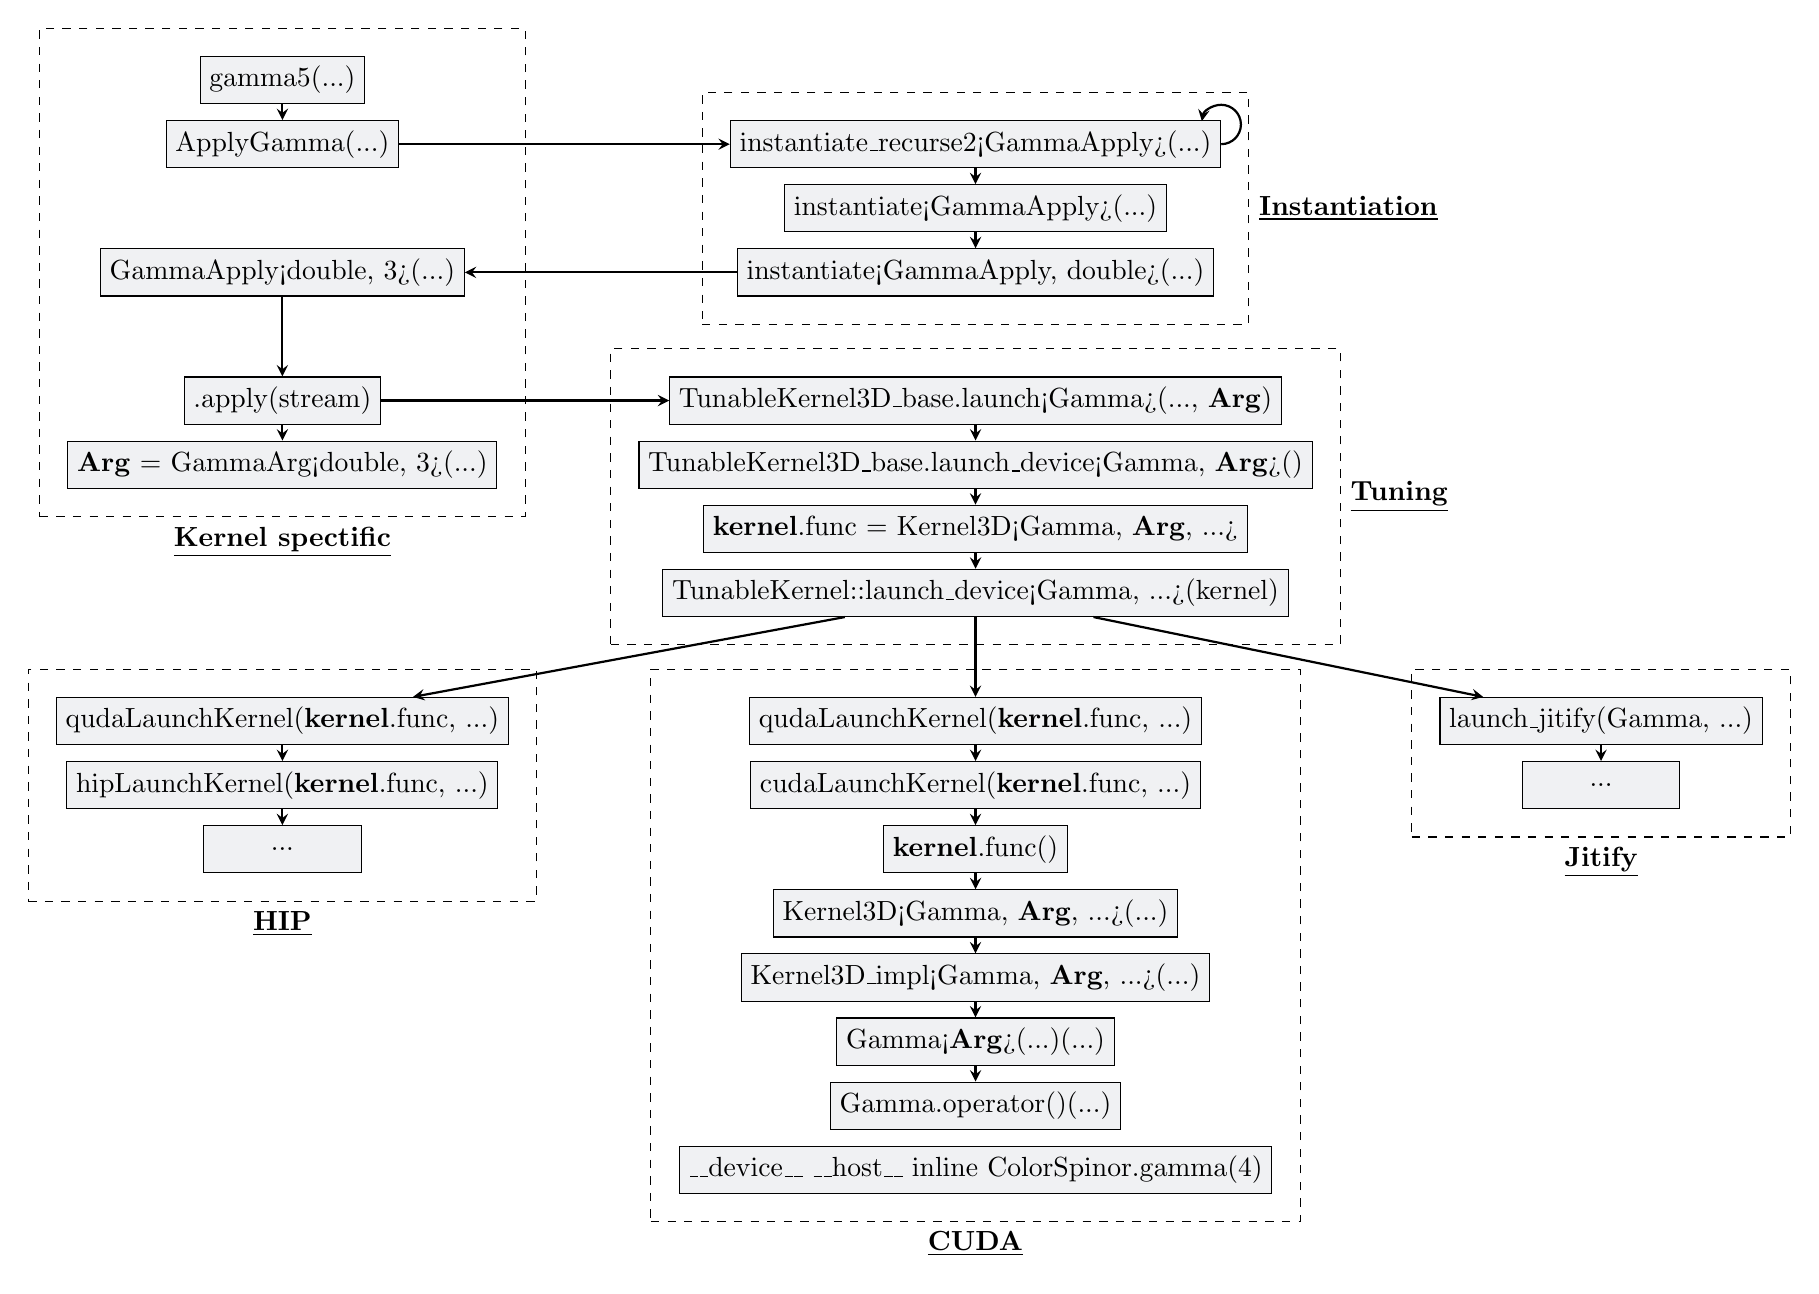
\begin{tikzpicture}[node distance=0.2cm, auto]

\node (gamma5) [process] {\edge{gamma5(...)}};
\node (ApplyGamma) [process, below=of gamma5] {\edge{ApplyGamma(...)}};
\node (recurse) [process, right=of ApplyGamma, xshift=4cm] {\edge{instantiate\_recurse2<GammaApply>(...)}};
\node (inst1) [process, below=of recurse] {\edge{instantiate<GammaApply>(...)}};
\node (inst2) [process, below=of inst1] {\edge{instantiate<GammaApply, double>(...)}};
\node (B1) [minimum height=0.6cm, below=of inst2] {};

\node (A1) [minimum height=0.6cm,below=of ApplyGamma] {};
\node (GammaApply) [process, below=of A1] {\edge{GammaApply<double, 3>(...)}};
\node (A0) [minimum height=0.6cm,below=of GammaApply] {};
\node (GammaApply2) [process, below=of A0] {\edge{.apply(stream)}};
\node (A2) [process,below=of GammaApply2] {\edge{\textbf{Arg} = GammaArg<double, 3>(...)}};
\node (A3) [minimum height=0.6cm,below=of A2] {};
\node (A4) [minimum height=0.6cm,below=of A3] {};
\node (A5) [minimum height=0.6cm,below=of A4] {};



\node (TunableKernel3D) [process, below=of B1] {\edge{TunableKernel3D\_base.launch<Gamma>(..., \textbf{Arg})}};

\node (TunableKernel3D2) [process, below=of TunableKernel3D] {\edge{TunableKernel3D\_base.launch\_device<Gamma, \textbf{Arg}>()}};
\node (Kernel3D) [process, below=of TunableKernel3D2] {\edge{\textbf{kernel}.func = Kernel3D<Gamma, \textbf{Arg}, ...>}};

\node (TunableKernel) [process, below=of Kernel3D] {\edge{TunableKernel::launch\_device<Gamma, ...>(kernel)}};
\node (B2) [minimum height=0.6cm, below=of TunableKernel] {};

\node (C1) [minimum height=0.6cm, right=of recurse, xshift=4.5cm] {};
\node (C2) [minimum height=0.6cm, below=of C1] {};
\node (C3) [minimum height=0.6cm, below=of C2] {};
\node (C4) [minimum height=0.6cm, below=of C3] {};
\node (C5) [minimum height=0.6cm, below=of C4] {};
\node (C6) [minimum height=0.6cm, below=of C5] {};
\node (C7) [minimum height=0.6cm, below=of C6] {};
\node (C8) [minimum height=0.6cm, below=of C7] {};
\node (C9) [minimum height=0.6cm, below=of C8] {};

\node (CUDA1) [process, below=of B2] {\edge{qudaLaunchKernel(\textbf{kernel}.func, ...)}};
\node (CUDA2) [process, below=of CUDA1] {\edge{cudaLaunchKernel(\textbf{kernel}.func, ...)}};
\node (CUDA3) [process, below=of CUDA2] {\edge{\textbf{kernel}.func()}};
\node (CUDA4) [process, below=of CUDA3] {\edge{Kernel3D<Gamma, \textbf{Arg}, ...>(...)}};
\node (CUDA5) [process, below=of CUDA4] {\edge{Kernel3D\_impl<Gamma, \textbf{Arg}, ...>(...)}};
\node (CUDA6) [process, below=of CUDA5] {\edge{Gamma<\textbf{Arg}>(...)(...)}};
\node (CUDA7) [process, below=of CUDA6] {\edge{Gamma.operator()(...)}};
\node (CUDA8) [process, below=of CUDA7] {\edge{\_\_device\_\_ \_\_host\_\_ inline ColorSpinor.gamma(4)}};

\node (HIP1) [process, below=of A5] {\edge{qudaLaunchKernel(\textbf{kernel}.func, ...)}};
\node (HIP2) [process, below=of HIP1] {\edge{hipLaunchKernel(\textbf{kernel}.func, ...)}};
\node (HIP3) [process, below=of HIP2] {\edge{...}};

\node (JIT1) [process, below=of C9] {\edge{launch\_jitify(Gamma, ...)}};
\node (JIT2) [process, below=of JIT1] {\edge{...}};

\node[draw, dashed, inner sep=10pt, label={below:\head{Kernel spectific}}] (group) 
  [fit={(gamma5) (ApplyGamma) (A1) (GammaApply) (GammaApply2) (A2)}] {};

\node[draw, dashed, inner sep=10pt, label={right:\head{Instantiation}}] (group) 
  [fit={(recurse) (inst1) (inst2)}] {};

\node[draw, dashed, inner sep=10pt, label={right:\head{Tuning}}] (group) 
  [fit={(TunableKernel3D) (TunableKernel3D2) (TunableKernel)}] {};

\node[draw, dashed, inner sep=10pt, label={below:\head{HIP}}] (group) 
  [fit={(HIP1) (HIP2) (HIP3)}] {};

\node[draw, dashed, inner sep=10pt, label={below:\head{CUDA}}] (group) 
  [fit={(CUDA1) (CUDA2) (CUDA3) (CUDA4) (CUDA5) (CUDA6) (CUDA7) (CUDA8)}] {};

\node[draw, dashed, inner sep=10pt, label={below:\head{Jitify}}] (group) 
  [fit={(JIT1) (JIT2)}] {};

\draw [arrow] (gamma5) -- (ApplyGamma);
\draw [arrow] (ApplyGamma) -- (recurse);
\draw [arrow] (recurse) -- (inst1);
\draw [arrow] (inst1) -- (inst2);
\draw [arrow] (inst2) -- (GammaApply);
\draw [arrow] (GammaApply) -- (GammaApply2);
\draw [arrow] (GammaApply2) -- (TunableKernel3D);
\draw [arrow] (GammaApply2) -- (A2);
\draw [arrow] (TunableKernel3D) -- (TunableKernel3D2);
\draw [arrow] (TunableKernel3D2) -- (Kernel3D);
\draw [arrow] (Kernel3D) -- (TunableKernel);

\draw[arrow] (recurse.east) arc (-90:170:2.5mm);

\draw [arrow] (TunableKernel) -- (HIP1);
\draw [arrow] (HIP1) -- (HIP2);
\draw [arrow] (HIP2) -- (HIP3);

\draw [arrow] (TunableKernel) -- (JIT1);
\draw [arrow] (JIT1) -- (JIT2);

\draw [arrow] (TunableKernel) -- (CUDA1);
\draw [arrow] (CUDA1) -- (CUDA2);
\draw [arrow] (CUDA2) -- (CUDA3);
\draw [arrow] (CUDA3) -- (CUDA4);
\draw [arrow] (CUDA4) -- (CUDA5);
\draw [arrow] (CUDA5) -- (CUDA6);
\draw [arrow] (CUDA6) -- (CUDA7);

% \node (pro2a) [process, below of=dec1] {Process 2a
% text text text text
% text text text 
% text text text};

% \node (pro2b) [process, right of=dec1, xshift=2cm] {Process 2b};
% \node (out1) [process, below of=pro2a] {Output};
% \node (stop) [process, below of=out1] {Stop};

% \draw [arrow] (gamma5) -- (ApplyGamma);
% \draw [arrow] (ApplyGamma) -- (recurse);
% \draw [arrow] (recurse) -- (dec1);
% \draw [arrow] (dec1) -- node[anchor=east] {yes} (pro2a);
% \draw [arrow] (dec1) -- node[anchor=south] {no} (pro2b);
% \draw [arrow] (pro2b) |- (recurse);
% \draw [arrow] (pro2a) -- (out1);
% \draw [arrow] (out1) -- (stop);

\end{tikzpicture}
\end{document}
